% Toolbar icon: fitCad — fit_mesh_to_cad: a mesh triangle replaced by the exact
% analytic surface it fits (segment -> fitPrimitives -> fitCad). Deliberately
% distinct from fit.tex (the view-fit camera action) and export.tex (the
% one-shot export tray "Promote to B-rep…" uses): the mesh-to-analytic pair
% reads left (the facet) to right (the circle the fit replaces it with).
\documentclass[tikz,border=2mm]{standalone}
\usetikzlibrary{arrows.meta,calc,shapes.geometric}
\begin{document}
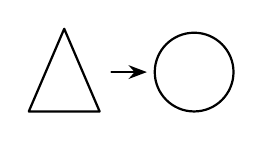
\begin{tikzpicture}[line width=1.3pt, line cap=round, line join=round, >=Stealth, x=1mm,y=1mm]
  \draw[thick] (-11.5,-6) -- (-7,4.5) -- (-2.5,-6) -- cycle;
  \draw[->, thick] (-1,-1) -- (3.5,-1);
  \draw[thick] (9.5,-1) circle (5);
\end{tikzpicture}
\end{document}
